\chapter{Implementacja}
    W rozdziale tym przedstawiono proces implementacji projektu. Najpierw opracowano moduł \emph{XBit}, następnie \emph{Z80emu{\dywiz}core} i~na końcu \emph{Z80emu{\dywiz}gui}. Implementację każdego z~nich opisano w osobnym podrozdziale. Zaprezentowano najciekawsze fragmenty kodu źródłowego i je opisano. 

	\section{XBit}

\emph{XBit} to moduł mający za zadanie ułatwić operacje bitowe w języku Java, która interpretuje liczby całkowite w kodzie dopełnień do dwóch i nie jest możliwa interpretacja ich w naturalnym kodzie binarnym (w skrócie NKB). Z tego powodu powstał moduł \emph{XBit} implementujący taką operację. Potrafi on odczytać liczbę n{\dywiz}bitową i zwrócić jej wartość jako zmienną typu \emph{int}, interpretując ją jako bity w U2 lub NKB.


Wewnątrz obiektów reprezentujących liczby binarne, wartość przechowywana jest w~polu typu \emph{int}, które nazwano \emph{valueContainer}. Może ono przyjąć teoretycznie wartości od -2147483648 do 2147483647. Uznano jednak, że atrybut ten przechowywał będzie wartość, jaką reprezentują przechowywane bity w notacji NKB (czyli tylko wartości dodatnie). Z tego powodu wartość \emph{valueContainer} nigdy nie będzie ujemna. \newline
Zakres wartości tego pola to od 0 do $ 2^{n}-1, n<32 $ gdzie \emph{n} oznacza liczbę bitów, jaką przechowuje dany obiekt. Ponieważ typ \emph{int} przechowywany jest w czterech bajtach i interpretowany jest przez język Java w notacji U2, maksymalnie może przechować wartość 2 147 483 647. Dla wartości interpretowanej w NKB na czterech bajtach jest to \newline $2^{32}-1 =$ 4 294 967 296. Jest to więcej niż typ \emph{int} może zawierać, dlatego maksymalna możliwa binarna reprezentacja, jaka może zostać zapisana w podobny sposób, to liczba przechowywana na 31 bitach.

Jeśli obiekt \emph{XBit8} będzie przechowywał liczbę binarną 11111111 (czyli odczytując w~NKB to decymalne 255, a w U2 decymalnie -1). Wartość jego pola \emph{valueContainer} będzie wynosić w~kodzie binarnym
00000000 00000000 00000000 11111111. (czyli odczytując zarówno w NKB, jak i w U2 będzie to 255). Niestety nadmiarowość bitów jest w tym rozwiązaniu wymagana, ponieważ liczba w kodzie U2, której najbardziej znaczący bit ma wartość $1$, jest ujemna. 

Podsumowując, \emph{XBit} wykorzystuje fakt takiego samego zapisu liczb dodatnich w U2 i NKB, jeśli tylko będą one zapisane na większej liczbie bitów niż wymagana.


\subsection{Implementacja klasy \emph{XBit}}
\emph{XBit} to klasa abstrakcyjna zawierająca wspólne elementy dla klas \emph{XBit8} i \emph{XBit16} oraz, ewentualnych klas dziedziczących.W~tym podrozdziale zawarto opis najbardziej istotnych metod tej klasy.

\subsubsection{boolean getBit(int index)}

\begin{listing}[h]
	\inputminted{java}{listings/xbit/xbitMethodGetBit.java}
	\caption{Metoda boolean getBit(int index)}
	\label{listing:xbitMethodGetBit}
\end{listing}
Na listingu \ref{listing:xbitMethodGetBit} zaprezentowano metodę \emph{getBit} zwracającą wartość bitu na pozycji o~numerze przekazanym w parametrze. W linii nr 2 sprawdzana jest poprawność parametru \emph{index}. Jeśli jest on niepoprawny, w linii nr 3 wyrzucany jest wyjątek \emph{NumberFormatException}. W linii nr 5 metoda wykonuje przesunięcie bitowe pola \emph{valueContainer} o~podany index. Ponieważ wynikiem jest liczba o typie \emph{int}, wykonywana zostaje koniunkcja bitowa z maską o wartości 1. Na końcu wynik operacji jest przekształcany z typu \emph{int} na \emph{boolean} i zwracany.


\subsubsection{setBit(int index, boolean value)}
\begin{listing}[h]
	\inputminted{java}{listings/xbit/xbitMethodSetBit.java}
	\caption{Metoda TSelf setBit(int index, boolean value)}
	\label{listing:xbitMethodSetBit}
\end{listing}	
Listing \ref{listing:xbitMethodSetBit} prezentuje metodę nadającą bitowi o określonej pozycji, zadaną wartość, a~następnie zwracającą nowy zmodyfikowany obiekt. Typ \emph{TSelf} zwracanej wartości to typ generyczny reprezentujący docelową liczbę n-bitową. W linii nr 2 metoda tworzy maskę bitową, wykonując przesunięcie bitowe na liczbie 1 o wartość parametru \emph{index}, czyli maska będzie posiadała tylko jeden bit ustawiony na wartość $1$, i będzie to bit o~pozycji z~parametru. W liniach 5 i 7 metoda wykonuje operacje bitowe mające na celu zmianę bitu na 1 lub 0 w zależności od parametru \emph{value}:
\begin{itemize}  
	\item dla \emph{value} równego 1 wykonywane są instrukcje zawarte w~linii nr~5. Najpierw pobierana jest obecna wartość obiektu i wykonana alternatywa bitowa  na niej i na wcześniej zbudowanej masce. Metoda przypisuje wynik do zmiennej \emph{newValue} będącej buforem,
	\item dla \emph{value} równego 0 metoda wykonuje instrukcje zawartą w linii nr~7. Nowa wartość uzyskiwana jest przez koniunkcje bitową aktualnej wartości oraz negacji maski. 
\end{itemize} 

\subsubsection{int getValueOfBits(int startIndexBit, int stopIndexBit)}
\begin{listing}[h]
	\inputminted{java}{listings/xbit/getValueOfBits.java}
	\caption{Metoda int getValueOfBits(int startIndexBit, int stopIndexBit)}
	\label{listing:getValueOfBits}
\end{listing}
Listing \ref{listing:getValueOfBits} przedstawia metodę zwracającą fragment wartości binarnej, od pozycji określonej przez argument \emph{startIndexBit}. do \emph{stopIndexBit}, włącznie.

W liniach 2 i 3 sprawdzana jest poprawność argumentów i ewentualnie zostaje wyrzucony wyjątek.  W linii 6 tworzony jest bufor, wykonując przesunięcie bitowe w prawo na wartości obiektu, o wartość parametru \emph{stopIndexBit}. Dzięki tej operacji pozbyto się zbędnych bitów z wartości obiektu po prawej stronie. Następnym krokiem jest pozbycie się bitów po lewej stronie. W tym celu, w linii nr 7 wykonywana jest maska bitowa wypełniona taką liczbą jedynek, jak liczba bitów docelowej wartości. Aby ją wykonać, wykonujemy przesunięcie bitowe w lewo na maksymalnej liczbie, jaką może przyjąć typ \emph{int} (w zapisie binarnym 01111111 11111111 11111111 11111111) o liczbę bitów wartości docelowej - 1. Następnie wykonano negację bitową. Bitów po lewej stronie pozbyto się za pomocą operacji iloczynu bitowego na uzyskanej masce i buforze.

\subsubsection{Inne metody}
Klasa \emph{XBit} posiada inne metody, zbyt proste w swojej budowie, aby były warte dokładniejszego opisywania. Zostaną one jedynie wymienione w celu lepszego zobrazowania wszystkich możliwości.
\begin{itemize}  
	\item \emph{public abstract short getSize()} - abstrakcyjna metoda zwracająca liczbę bitów jakie przechowuje docelowa liczba,
	\item \emph{public abstract int getMinSignedValue()} - zwraca minimalną liczbę ze znakiem jaka może być przechowywana w obiekcie,
	\item \emph{public abstract int getMaxSignedValue()} - zwraca maksymalną liczbę ze znakiem jaka może być przechowywana w obiekcie,
	\item \emph{public int getMinUnsignedValue()} - zwraca minimalną liczbę bez znaku jaka może być przechowywana w obiekcie (czyli zawsze przyjmuje wartość 0),
	\item \emph{public abstract int getMaxUnsignedValue()} - zwraca maksymalną liczbę bez znaku jaka może być przechowywana w obiekcie,
	\item \emph{public boolean isNegative()} - zwraca wartość bitu o największej pozycji, który w kodowaniu U2 decyduje czy liczba jest mniejsza od zera,
	\item \emph{public int getSignedValue()} - zwraca wartość w kodowaniu U2,
	\item \emph{public int getUnsignedValue()} - zwraca wartość w kodowaniu NKB.
\end{itemize}

\subsection{Implementacja klasy \emph{XBit8}}
Klasa \emph{XBit8} dziedziczy po abstrakcyjnej klasie \emph{XBit}, która została zbudowana w taki sposób, aby klasy po niej dziedziczące były jak najmniejsze. Metody, które należą do \emph{XBit8} i nie zostały odziedziczone. Nie są one na tyle skomplikowane, aby warto było je bardziej szczegółowo opisywać, z tego powodu zostaną wymienione i krótko opisane.
\begin{itemize}  
	\item \emph{public static XBit8 valueOfUnsigned(int value)} - tworzy nowy obiekt o wartości bez znaku,
	\item \emph{public static XBit8 valueOfSigned(int value)} - tworzy nowy obiekt o wartości ze znakiem,
	\item \emph{public static XBit8 valueOfBooleanArray(boolean[] values)} - tworzy nowy obiekt na podstawie tablicy elementów o typie \emph{boolean}.
\end{itemize}

\subsection{Implementacja klasy XBit16}
\emph{XBit16} to klasa reprezentująca liczbę 16 bitową. Dziedziczy ona po \emph{XBit}. Dzięki temu nie musi implementować najbardziej podstawowych metod. 


\subsubsection{public static XBit16 valueOfHighAndLowInBigEndian(XBit8 high, XBit8 low)}
\begin{listing}[h]
	\inputminted{java}{listings/xbit/valueOfHighAndLowInBigEndian.java}
	\caption{Metoda XBit16 valueOfHighAndLowInBigEndian(XBit8 high, XBit8 low)}
	\label{listing:valueOfHighAndLowInBigEndian}
\end{listing}
Listingu \ref{listing:valueOfHighAndLowInBigEndian} przedstawia implementację metody \emph{valueOfHighAndLowInBigEndian} tworzącej liczbę 16{\dywiz}bitową w formacie zapisu \emph{big endian} (najbardziej znaczący bajt umieszczony jest jako pierwszy). Przyjmuje ona jako parametry dwie liczby 8{\dywiz}bitowe o nazwach \emph{high} i \emph{low}. 
Metoda tworzy obiekt klasy \emph{ByteBuffer} należącej do standardowej biblioteki języka Java i konfiguruje ją, aby przechowywała dane w formacie \emph{big endian} (linia nr 3). 
Następne linie prezentują operacje dodania do bufora kolejno starszego (linia nr 4) i~młodszego  bajtu (linia nr 5). Na koniec wykonano metodę \emph{getShort()} zwracającą docelową liczbę i na jej podstawie tworzona jest reprezentacja klasy \emph{XBit16}.

\subsubsection{public static XBit16 valueOfHighAndLowInLittleEndian(XBit8 high, XBit8 low)}
\begin{listing}[h]
	\inputminted{java}{listings/xbit/valueOfHighAndLowInLittleEndian.java}
	\caption{Metoda XBit16 valueOfHighAndLowInLittleEndian(XBit8 high, XBit8 low)}
	\label{listing:valueOfHighAndLowInLittleEndian}
\end{listing}
W listingu \ref{listing:valueOfHighAndLowInLittleEndian} zaprezentowano metodę tworzącą liczbę 16{\dywiz}bitową w formacie zapisu \emph{little endian}, czyli najbardziej znaczący bajt umieszczony jest jako ostatni.
Implementacja metody jest dosyć prosta, wykonuje ona metodę \emph{valueOfHighAndLowInBigEndian()} z~zamienioną kolejnością parametrów.


\subsubsection{Inne metody}
Klasa \emph{XBit16} zawiera także metody, które są zbyt proste w implementacji aby warto było je opisywać pojedynczo:
\begin{itemize}  
	\item \emph{public static XBit16 valueOfUnsigned(int value)} - tworzy nowy obiekt o wartości bez znaku,
	\item \emph{public static XBit16 valueOfSigned(int value)} - tworzy nowy obiekt o wartości ze znakiem.
\end{itemize}


\subsection{Implementacja klasy XbitUtils}
\emph{XbitUtils} to klasa implementująca operacje arytmetyczne i bitowe na obiektach \emph{XBit8} i~\emph{XBit16}. Posiada ona dwie klasy wewnętrzne, \emph{Arithmetic8bitResult}  oraz \newline\emph{Arithmetic16bitResult} reprezentujące wynik operacji arytmetycznych i zawierające informacje o wystąpieniu przeniesienia i przepełnienia. Klasy te zaprezentowano w listingach \ref{listing:arithmetic8bitResult} oraz \ref{listing:arithmetic16bitResult}.

\begin{listing}[h]
	\inputminted{java}{listings/xbit/arithmetic8bitResult.java}
	\caption{Klasa Arithmetic8bitResult}
	\label{listing:arithmetic8bitResult}
\end{listing}

\begin{listing}[h]
	\inputminted{java}{listings/xbit/arithmetic16bitResult.java}
	\caption{Klasa Arithmetic16bitResult}
	\label{listing:arithmetic16bitResult}
\end{listing}

\subsubsection{public static XBit8 incrementBy(XBit8 value, int incrementer)}
\begin{listing}[h]
	\inputminted{java}{listings/xbit/incrementBy.java}
	\caption{Metoda XBit8 incrementBy(XBit8 value, int incrementer)}
	\label{listing:incrementBy}
\end{listing}
Listing \ref{listing:incrementBy} prezentuje metodę zwiększającą liczbę 8{\dywiz}bitową o daną wartość. Aby wykonać operację, metoda konwertuje parametr \emph{value} na liczbę typu \emph{int} (linia nr 2) i dodaje wartość parametru \emph{incrementer} (linia nr 3). Następnie w linii nr 4 wykonuje operacje iloczynu bitowego na uzyskanej nowej wartości oraz masce bitowej reprezentującej największą możliwą wartość, jaką może przechowywać liczba 8{\dywiz}bitowa (celem tej operacji jest niedopuszczenie do sytuacji, w której wynik operacji nie mieści się na ośmiu bitach). Na koniec tworzona jest i zwracana instancja klasy \emph{XBit8}. 

Zasada działania metody \emph{XBit16 incrementBy(XBit16 value, int incrementer)} jest podobna, dlatego jej opis zostanie pominięty. 

\subsection{public static XBit8 negativeOf(XBit8 value)}
\begin{listing}[h]
	\inputminted{java}{listings/xbit/negativeOf.java}
	\caption{Metoda XBit8 negativeOf(XBit8 value)}
	\label{listing:negativeOf}
\end{listing}
Funkcja tworząca liczbę o~przeciwnym znaku do podanej została zaprezentowana w~listingu \ref{listing:negativeOf}. Operacja ta polega na wykonaniu iloczynu bitowego na negacji bitowej danej wartości oraz liczbie 255. Ma to na celu niedopuszczenie do sytuacji, w której wartość bufora będzie większa niż 255, a więc nie będzie mogła się zmieścić na ośmiu bitach.
Następnie wykonany wynik zostaje zwiększony o jeden. 

Zasada działania metody \emph{XBit16 negativeOf(XBit16 value)} jest taka sama. Jedyną różnicą jest operacja iloczynu bitowego, którą wykonujemy nie na liczbie 255 a 65535.

\subsection{public static Arithmetic8bitResult addTwo8bits(XBit8 value1, XBit8 value2)}
\begin{listing}[h]
	\inputminted{java}{listings/xbit/addTwo8bits.java}
	\caption{Metoda Arithmetic8bitResult addTwo8bits(XBit8 value1, XBit8 value2)}
	\label{listing:addTwo8bits}
\end{listing}
Listing \ref{listing:addTwo8bits} prezentuje metodę realizującą dodawanie dwóch liczb 8-bitowych. Wynikiem jej działania jest obiekt klasy \emph{Arithmetic8bitResult} przechowujący wynik operacji i flagi przepełnienia lub przeniesienia. 

W linii nr 3 metoda wykonuje operacje dodawania. W linii nr 4 umieszczono sprawdzenie, czy nastąpiło przepełnienie, a linia nr 5 ustawia flagę. Linia nr 7 wykonuje ,,obcięcie" bitów w przypadku, gdy wynik nie będzie w stanie zmieścić się w liczbie 8{\dywiz}bitowej.

Linie 9 i 10 zawierają operację ustawiającą flagę przepełnienia według\newline trzech zasad \cite{overflowRules}:
\begin{enumerate}
	\item jeśli suma dwóch liczb dodatnich daje wynik ujemny, to znaczy, że wystąpiło przepełnienie,
	\item jeśli suma dwóch liczb ujemnych daje wynik dodatni, to również oznaca wystąpienie przepełnienia,
	\item w każdym innym przypadku przepełnienie nie wystąpiło.
\end{enumerate}
Zakłada się, że najbardziej znaczący bit jest bitem znaku.

Prezentacja metody realizującej dodawanie dwóch liczb 16{\dywiz}bitowych została pominięta, ponieważ operacja ta jest przeprowadzana na tej samej zasadzie co 8{\dywiz}bitowa.

\subsection{public static Arithmetic8bitResult subTwo8bits(XBit8 value1, XBit8 value2)}
\begin{listing}[h]
	\inputminted{java}{listings/xbit/subTwo8bits.java}
	\caption{Metoda Arithmetic8bitResult subTwo8bits(XBit8 value1, XBit8 value2)}
	\label{listing:subTwo8bits}
\end{listing}
W listingu \ref{listing:subTwo8bits} zaprezentowano metodę realizującą odejmowanie jednej liczby 8{\dywiz}bitowej, od drugiej. Metoda wykorzystuje regułę 
$ a - b = a+(-b) $ według której odejmowanie dwóch liczb można zastąpić dodawaniem, negując drugi składnik odejmowania. 
Metoda realizująca odejmowanie dwóch liczb 16{\dywiz}bitowych działa w analogiczny sposób.

\subsection{public static XBit8 not8bit(XBit8 value)}
\begin{listing}[h]
	\inputminted{java}{listings/xbit/not8bit.java}
	\caption{Metoda XBit8 not8bit(XBit8 value)}
	\label{listing:not8bit}
\end{listing}
Metoda \emph{not8bit(XBit8 value)} zaprezentowana w listingu \ref{listing:not8bit} wykonuje negację bitową na liczbie 8{\dywiz}bitowej. Operacja wykonywana jest za pomocą standardowego operatora negacji bitowej języka Java (znak tyldy górnej ,,\~{}"). Dodatkową wykonywaną operacją jest iloczyn bitowy z liczbą 255, mający za zadanie wyzerowanie bitów starszych od ósmego. Wersja metody dla liczb 16{\dywiz}bitowych jest analogiczna.

\subsection{public static XBit8 and8bit(XBit8 value1, XBit8 value2)}
\begin{listing}[h]
	\inputminted{java}{listings/xbit/and8bit.java}
	\caption{Metoda XBit8 and8bit(XBit8 value1, XBit8 value2)}
	\label{listing:and8bit}
\end{listing}
Listing \ref{listing:and8bit} prezentuje metodę wykonującą operację sumy logicznej dwóch liczbe \mbox{8{\dywiz}bitowych} (linia nr 3). Linia nr 4 zawiera operację wyzerowania bitów starszych od ósmego dla wyniku, aby mieścił się on w ośmiu bitach. Wersja metody dla liczb \mbox{16{\dywiz}bitowych} działa analogicznie.

\subsection{Metody wykonujące sumę bitową i różnice symetryczną}
Implementacje metod:
\begin{itemize}  
	\item \emph{public static XBit8 or8bit(XBit8 value1, XBit8 value2)},
	\item \emph{public static XBit16 or16bit(XBit16 value1, XBit16 value2)},
	\item \emph{public static XBit8 xor8bit(XBit8 value1, XBit8 value2)},
	\item \emph{public static XBit16 xor16bit(XBit16 value1, XBit16 value2)},
	\item \emph{public static XBit8 shift8bit(XBit8 value1, int position)},
	\item \emph{public static XBit8 shift16bit(XBit8 value1, int position)}.
\end{itemize}
są analogicznie do metody and8bit(XBit8 value1, XBit8 value2). Operacje bitowe wykonywane są za pomocą mechanizmów wbudowanych w język Java, a nadmiar bitów zostaje obcięty.
	\section{Z80emu-core}
Z80emu-core to moduł mający za zadanie wykonać proces emulacji. Używa on do swojego działania bibliotekę XBit.

@todo tutaj podział na pakiety

\subsection{obiekt klasy Z80}

\subsection{opis registerbank}

\subsection{opis flagmanager}

\subsection{opis memory}

\subsection{opis io}

\subsection{InstructionDecoder i instructionContainer}

\subsection{opis instrukcje}

\subsection{opis helpery do instrukcji}

	\section{Z80emu{\dywiz}gui}

Moduł \emph{Z80emu{\dywiz}gui} implementuje interfejs użytkownika zaprezentowany na rysunku nr \ref{img:z80Gui}. Został on napisany z pomocą biblioteki \emph{JavaFX}. Największą jej zaletą w porównaniu do poprzedniczki, którą była biblioteka \emph{Swing}, jest możliwość definiowania widoku aplikacji za pomocą języków XML i CSS. Projektowanie interfejsu w \emph{JavaFx} przypomina nieco tworzenie strony WWW.

Kod źródłowy implementujący interfejs użytkownika został podzielony na pakiety, których strukturę przedstawiono na rysunku \ref{img:z80EmuGuiPackage}. Postanowiono podzielić pliki zgodnie ze wzorcem \emph{Model-View-Controller}, który dzieli aplikacje na trzy główne części. Każda z~nich ma swoją reprezentację w module jako oddzielna paczka:
\begin{itemize}
    \item \emph{model} - implementuje logikę biznesową. W tym przypadku, między innymi zarządza procesem asemblacji i emulacji.
    \item \emph{View} - opisuje widok aplikacji. W projektach zbudowanych za pomocą \emph{javaFx} są to pliki XML i CSS. Oprócz nich mogą też być pliki języka Java, odpowiedzialne za prezentację danych. W opisywanym projekcie są to np. klasy, których zadaniem jest kolorowanie składni w edytorze kodu asemblera, tworzenie okien dialogowych lub system pomocy.
    \item \emph{controller} - zadaniem kontrolera jest przetworzenie informacji od użytkownika, by na jej podstawie wywoływać metody modelu i aktualizować widok. W projekcie każda część interfejsu posiada osobny kontroler (dla przykładu, osobne kontrolery zajmują się pamięcią programu, przerwaniami, i edytorem kodu asemblera).
\end{itemize}

\begin{figure}[h]
		\centering
		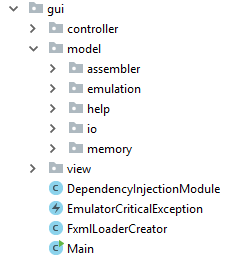
\includegraphics[width=0.4\textwidth]{z80EmuGuiPackage}
		\caption{Podział na pakiety modułu z80emu{\dywiz}gui}
		\label{img:z80EmuGuiPackage}
\end{figure}



\subsection{Wstrzykiwanie zależności za pomocą biblioteki \emph{Guice}}
Wstrzykiwanie zależności (z ang. \emph{Dependency Injection}) to technika programowania, której głównym założeniem jest przekazywanie gotowych skonfigurowanych już obiektów do innych (wstrzykiwanie ich), które ich wymagają. Moduł interfejsu użytkownika posiada wiele współpracujących ze sobą  klas. Zarządzanie nimi stało się z czasem uciążliwe. Problem postanowiono rozwiązać z pomocą biblioteki \emph{Guice}, która implementuje technikę wstrzykiwania zależności.

Aby opisać problem, należy przedstawić, z jakich elementów zostały zbudowane kontrolery w projekcie. Fragment jednego z nich został zaprezentowany w listingu \ref{listing:z80DiCOntrollerExample}. Kontroler ten jest zależny od modelu (linie nr 3-5) oraz posiada obiekty wstrzykiwane przez bibliotekę graficzną na podstawie plików FXML (linie nr 7 i 8). Zatem należało użyć biblioteki \emph{Guice} nie wprowadzając przy tym konfliktów z \emph{JavaFX}.

\begin{listing}[h]
	\inputminted{java}{listings/z80emu-gui/DiControllerExample.java}
	\caption{Zależności klasy \emph{MemoryController}}
	\label{listing:z80DiCOntrollerExample}
\end{listing}

Połączono \emph{JavaFx} i \emph{Guice} w następujący sposób. Interfejs biblioteki graficznej posiada metodę \emph{setControllerFactory(Callback<Class<?>, Object> controllerFactory)}, potrafiącą podmienić domyślną fabrykę kontrolerów. Jako jej parametr przekazano metodę biblioteki \emph{Guice} \emph{<T> T getInstance(Class<T> type)}, która zwraca instancję danego obiektu. Dzięki takiemu rozwiązaniu, kontrolery mają możliwość używania wszystkich adnotacji ułatwiających wstrzykiwanie do nich zależności (a nawet innych kontrolerów) i jednocześnie są udekorowane w~obiekty biblioteki graficznej.

\subsection{Integracja z projektem Z80emu{\dywiz}core}

\begin{listing}[h]
	\inputminted{java}{listings/z80emu-gui/EmulatorThread.java}
	\caption{Klasa \emph{EmulatorThread} realizująca emulację w trybie ciągłym}
	\label{listing:emulatorThread}
\end{listing}

\emph{Z80emu{\dywiz}gui} używa do emulacji modułu \emph{Z80emu{\dywiz}core}, który zawiera metodę \emph{runOneInstruction} wykonującą kolejną instrukcję CPU. Pomiędzy jej kolejnymi wywołaniami powinny zostać zgłoszone przerwania lub odczytane wartości rejestrów, pamięci i flag. Aby umożliwić to zarówno w trybie ciągłym, jak i krokowym wymagane było umieszczenie emulacji w osobnym wątku.

W tym celu wykonano klasę \emph{EmulatorThread}, którą pokazano w listingu \ref{listing:emulatorThread}. Użytkownik może uruchomić i zatrzymać emulację w dowolnym momencie za pomocą publicznych metod \emph{pause} i \emph{unPause}.

Metoda \emph{pause}, która docelowo zostaje wywoływana z innego wątku, zmienia wartość pola \emph{pause} typu \emph{boolean} na \emph{false}.  W głównej pętli emulacji sprawdzany jest warunek \emph{if(pause) \{lock.wait(); pause = false;\}}. Jeśli jest on spełniony, to wątek jest wprowadzany w stan oczekiwania.

Metoda \emph{unPause}, która także wywoływana jest z innego wątku, odblokowuje wątek, i~pozwala wznowić emulację.

% pomysły co mogło by się znaleźć w tym dziale: 
% - o wątkach, jak zaimplementowałem debugowanie ciągłe

% - podział na kontrolery, że jest wiele kontrolerów a nie jeden główny
% - opisać, jak podpiąłem biblioteke asemblującą, wspomnieć że to nie jest moje dzieło
% - ?? opisać jak działają przerwania
% - 
% - w jaki sposób zaimplementowano wiki, że jest to rekurencja itp. Wspomnieć że pliki jar nie mają struktury katalogów, i nie da się w nich wylistować listy plików w danym katalogu, dlatego tak to skomplikowałem
% - info co zostało niepodpięte pod gui, np przerwania


	
	Implementacja przebiegła zgodnie z założonym projektem aplikacji. Stosunkowo najbardziej czasochłonną częścią implementacji, było opracowanie klas modułu \emph{Z80emu-core}, odpowiedzialnych za realizowanie rozkazów procesora. Spowodowane to było głównie ich ilością (158 instrukcji). Moduł \emph{XBit} spełnił swoje zadanie i znacznie uprościł kod źródłowy emulatora. 
	
	
	
	